% Especificaciones del tamaño de letra, tamaño de hoja, márgenes, librerias, etc.
\documentclass[12pt, letterpaper]{article}
\usepackage[english]{babel}
\usepackage[utf8]{inputenc}
\usepackage[T1]{fontenc}
\usepackage{mathrsfs}
\usepackage{amsmath}
\usepackage{graphicx}
\usepackage{subcaption}
\usepackage{hyperref}
\usepackage{url}
\usepackage{amssymb}
\usepackage{float}
\usepackage[framed, numbered]{matlab-prettifier}
%\usepackage[framed, numbered, autolinebreaks, useliterate]{mcode}
\usepackage[margin=1in]{geometry}
\renewcommand{\baselinestretch}{1.5}

% Enlace Bibliografía
\usepackage{csquotes}
\usepackage[notes,backend=biber]{biblatex-chicago}
\addbibresource{referencias.bib}

% Titulo, autores, fecha.
\title{Práctica \#8: Linealización del Sistema Dinámico}
\author{Carlos Vásquez 1155057}

% Inicio del documento
\begin{document}
\maketitle

\section*{Introducción}

La linealización de modelos matemáticos que representan sistemas dinámicos son de gran ayuda ya que nos permiten realizar aproximaciones a estos sistemas de manera que nos sea más fácil analizar el comportamiento de los mismos, aplicando métodos lineales.

El método que utilizaremos para linealizar el sistema es asumir que el mismo toma esta forma característica:

\begin{equation}
	\begin{split}
		\dot x &= \textbf{J}x\\
		\begin{bmatrix} 
			\dot x_{1} \\
			\dot x_2 \\
			\vdots \\
			\dot x_n
		\end{bmatrix} &=
		\textbf{J} \begin{bmatrix}
			x_1 \\
			x_2 \\
			\vdots \\
			x_n
		\end{bmatrix}
	\end{split}
\end{equation}
Donde A es la matriz Jacobiana definida como:

\begin{equation}
	\textbf{J} =
	\begin{bmatrix}
		\frac{\partial{\dot x_1}}{\partial{x_1}} & \frac{\partial{\dot x_1}}{\partial{x_2}} & \dots & \frac{\partial{\dot x_1}}{\partial{x_n}} \\

		\frac{\partial{\dot x_2}}{\partial{x_1}} & \frac{\partial{\dot x_2}}{\partial{x_2}} & \dots & \frac{\partial{\dot x_2}}{\partial{x_n}} \\

		\vdots & \vdots & \ddots & \vdots \\

		\frac{\partial{\dot x_n}}{\partial{x_1}} & \frac{\partial{\dot x_n}}{\partial{x_2}} & \dots & \frac{\partial{\dot x_n}}{\partial{x_n}} \\
	\end{bmatrix}
\end{equation}
Y es evaluada en el estado inicial en que se encuentren $x_1, x_2, \dots, x_n$

Como ejemplo podemos tomar el siguiente sistema dinámico:
\begin{equation}
	\begin{split}
		\dot x_1 &= x_2 \\
		\dot x_2 &= -a \sin(x_1) - bx_2
	\end{split}
\end{equation}

Si asumimos que el espacio de estado para este sistema está dado por $x_1 = 0$ y $x_2 = 0$, entonces al momento de evaluar la matriz Jacobiana obtendremos el siguiente resultado:

\begin{equation}
	\begin{split}
		\textbf{J} &=
	\begin{bmatrix}
		0 & 1 \\
		-a \cos(x_1) & -b
	\end{bmatrix} \Biggr \rvert_{x_1 = 0,\  x_2 = 0} \\
		\textbf{J} &=
	\begin{bmatrix}
		0 & 1 \\
		-a & -b
	\end{bmatrix}
	\end{split}
\end{equation}

Y por tanto nuestro sistema linealizado tomará la forma de la ecuación 1.

\begin{equation}
	\begin{split}
	\begin{bmatrix}
		\dot x_1 \\
		\dot x_2
	\end{bmatrix}
		&=
	\begin{bmatrix}
		0 & 1 \\
		-a & -b
	\end{bmatrix}
	\begin{bmatrix}
		x_1 \\
		x_2
	\end{bmatrix} \\
		\begin{bmatrix}
			\dot x_1 \\
			\dot x_2
		\end{bmatrix}
		&=
		\begin{bmatrix}
			x_2 \\
			-ax_1 - bx_2
		\end{bmatrix}
	\end{split}
\end{equation}
Ajustándo el sistema a la forma de la ecuación 3 obtenemos:
\begin{equation}
	\boxed{\begin{split}
		\dot x_1 &= x_2 \\
		\dot x_2 &= -ax_1 - bx_2
	\end{split}}
\end{equation}

Si comparamos la ecuación 3 con la ecuación 6, podremos darnos cuenta que el término $\sin(x_1)$ desaparece y es reemplazado por el argumento $x_1$. Esto es intuitivamente satisfactorio ya que podríamos haber realizado la misma linealización utilizando aproximaciones mediante series de Taylor evaluadas en 0. Para este caso, podemos percatarnos que la aproximación a la que se llegó para linealizar el modelo fue $\sin(\theta) \approx \theta$.

\section*{Desarrollo}
Ahora bien, para probarnos que la linealización es bastante cercana al modelo no lineal, es preciso realizar una simulación. Esta simulación expondrá cómo se comportan ambos sistemas. Primeramente construimos los sistemas a través de las funciones de MATLAB:

\begin{figure}[H]
	\centering
	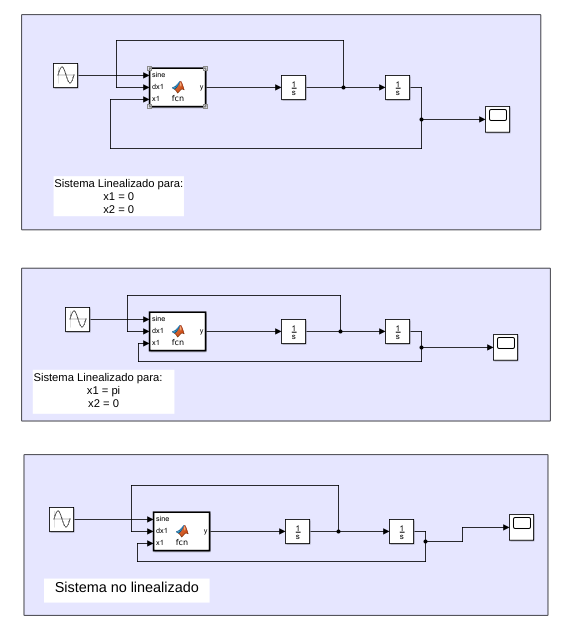
\includegraphics[width=0.8\textwidth]{systems.png}
	\caption{Los tres sistemas a analizar.}
\end{figure}

Como podemos observar, los sistemas son bastante sencillos, sin embargo hay 3 sistemas en lugar de los 2 sistemas de los que ya hemos hablado. Eso se debe a que un sistema linealizado está evaluado para $x_1 = \pi$ y $x_2 = 0$. Este estado resulta ser un punto inestable del sistema, así podremos visualizar lo que sucede cuando las condiciones iniciales toman estos valores.

Para los distintos sistemas tenemos los siguientes códigos (en orden):
\vspace{1cm}

\lstinputlisting[style=Matlab-editor, basicstyle=\mlttfamily\scriptsize, caption ={Código para $x_1 = 0$ y $x_2 = 0$ (linealizado).}]{./code/sin.m}

\lstinputlisting[style=Matlab-editor, basicstyle=\mlttfamily\scriptsize, caption ={Código para $x_1 = \pi$ y $x_2 = 0$ (linealizado).}]{./code/two.m}

\lstinputlisting[style=Matlab-editor, basicstyle=\mlttfamily\scriptsize, caption ={Código para sistema no linealizado..}]{./code/three.m}

Si deseamos, podemos analizar la manera en la que se comporta cada modelo si analizamos su posición. A continuación mostraremos las gráficas de posición de cada sistema.

\begin{figure}[H]
	\centering
	\begin{subfigure}[b]{0.49\linewidth}
		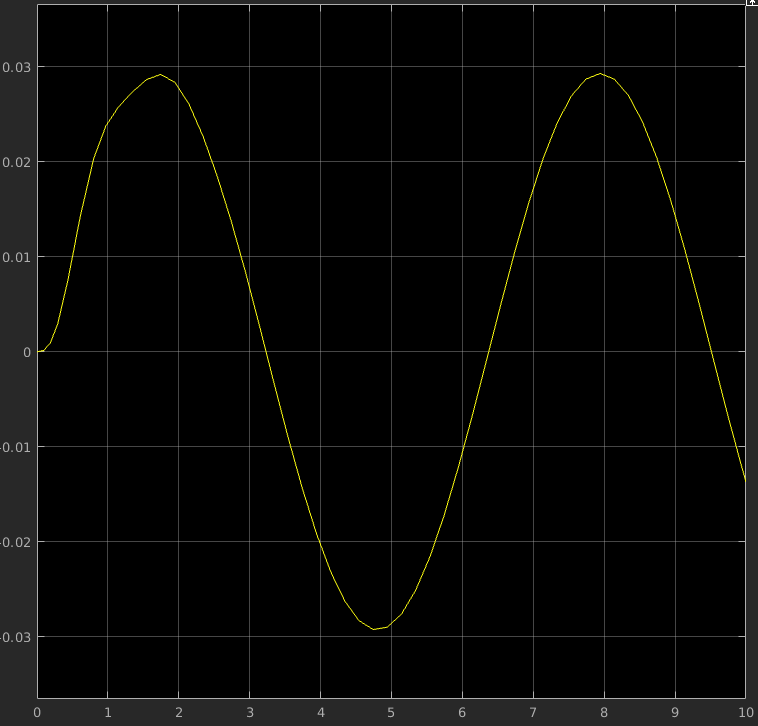
\includegraphics[width=\linewidth]{1.png}
		\caption{$x_1(t)$ para sistema lineal y $x_1 = 0$ y $x_2 = 0$.}
	\end{subfigure}
	\begin{subfigure}[b]{0.49\linewidth}
		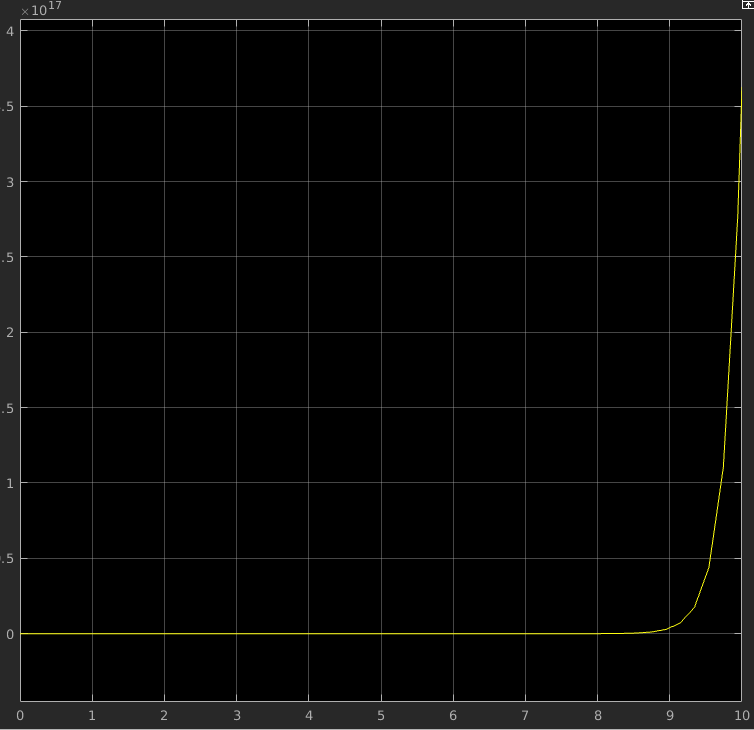
\includegraphics[width=\linewidth]{2.png}
		\caption{$x_1(t)$ para sistema lineal y $x_1 = \pi$ y $x_2 = 0$.}
	\end{subfigure}
	\begin{subfigure}[b]{0.49\linewidth}
		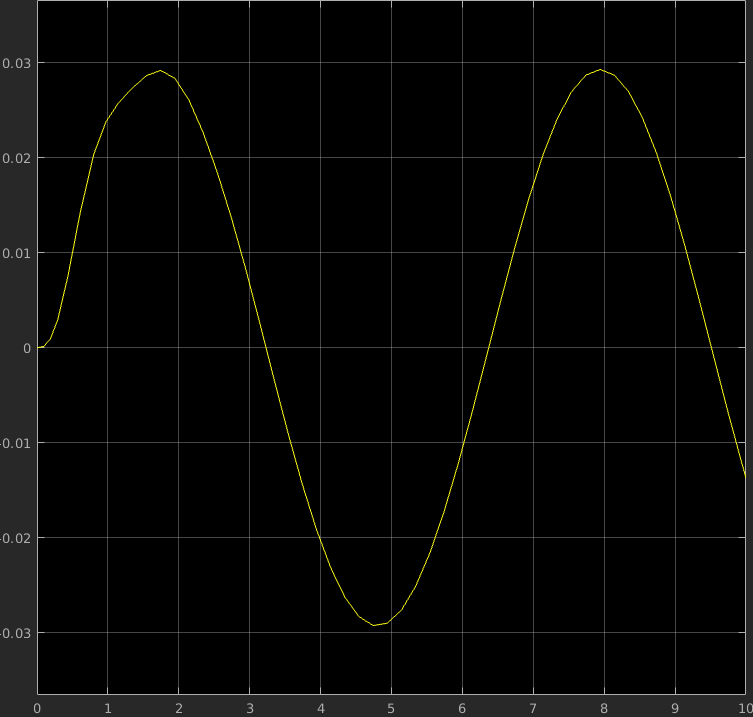
\includegraphics[width=\linewidth]{3.png}
		\caption{$x_1(t)$ para sistema no lineal.}
	\end{subfigure}
	\caption{Distintas gráficas de posiciones.}
\end{figure}

Como podemos observar, las gráficas de los modelos son estables, a excepción de la gráfica del sistema lineal cuyo estado inicial está dado por $x_1 = \pi$ y $x_2 = 0$. Intuitivamente, podemos pensar que el ángulo del péndulo es de $\pi$ radianes y la velocidad de 0 unidades, por lo que a lo largo del tiempo, sea la perturbación más mínima que exista, ésta desestabilizará al sistema y lo hará salir del punto fijo que es $(\pi,0)$.

\section*{Conclusión}

Después de haber visto cómo se comportan las gráficas, podemos concluir que aquella que representa la posición del sistema lineal y la otra que representa la del sistema con función senoidal son prácticamente las mismas, y a pesar de estar descritas de manera distinta, los errores son lo suficientemente pequeños como para asegurar la estabilidad en los puntos fijos que se encuentren en el sistema.
%%%%%  Bib
\renewcommand\refname{Referencias}
\printbibliography
\end{document}
